\setcounter{chapter}{5}

\chapter{定积分及其应用}

\section{定积分的概念与性质}




\section{微积分基本公式与定积分的计算}



\section{定积分的应用}

{\bf 定积分的构造思路──微元法:}

\begin{enumerate}
  \item {\bf 分割:}沿$x$轴方向分割曲边梯形 
  \item {\bf 取近似:}用小矩形的面积$\Delta S$近似小曲边梯形面积 
  \item {\bf 做和:}求所有小矩形的面积总和$\sum \Delta S$ 
  \item {\bf 求极限:}$\sum \Delta S\to S$
\end{enumerate}

\begin{center}
	\resizebox{!}{5.5cm}{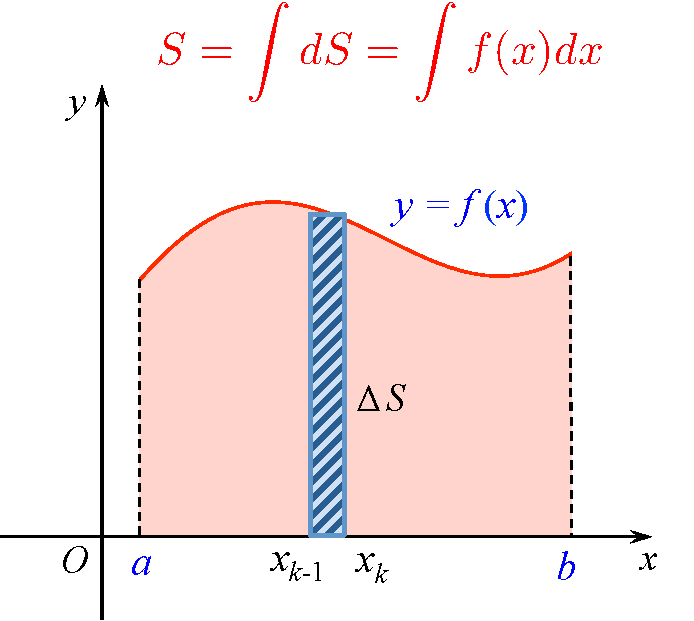
\includegraphics{./images/ch6/sumSSS.pdf}}
\end{center}

\subsection{几何应用}

\subsubsection{【面积】}

{\bf 例:}计算两条抛物线$y^2=x$和$y=x^2$所围图形的面积。

{\bf 例:}计算两条抛物线$y^2=2x$与直线$y=x-4$所围图形的面积。

{\bf 例:}推导圆和扇形的面积公式。

\subsubsection{【极坐标下的面积】}

{\bf 例:}计算Archimedes螺线$\rho=a\theta\;(a>0)$
相应于$\theta$从$0$变到$2\pi$的一段弧与极轴所围的图形面积。

\begin{center}
	\resizebox{!}{4cm}{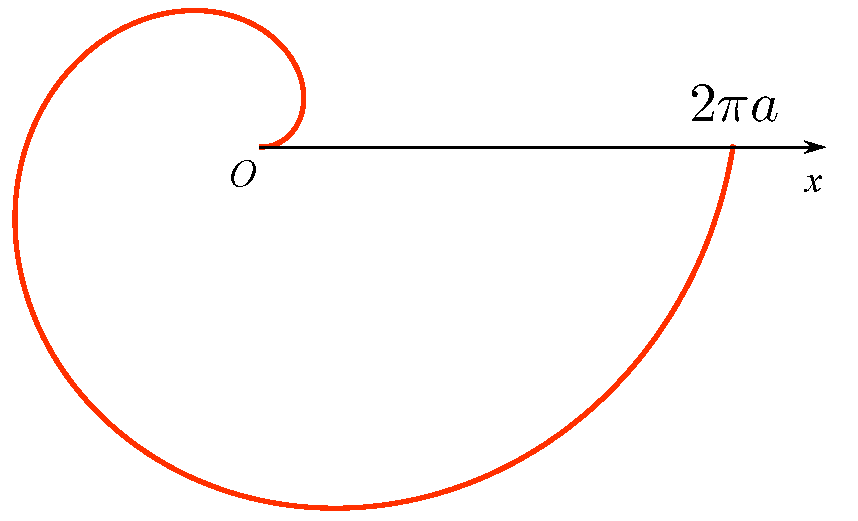
\includegraphics{./images/ch6/Achimedes.pdf}}
\end{center}

{\bf 例}(老羊三问题)
\begin{enumerate}[(1)]
  \setlength{\itemindent}{1cm}
  \item 半径为$a$的圆形水池,一只老羊被长为$ka(0<k\leq2)$的绳子拴在水池边缘,求
  老羊能吃到的草地面积
  \item 如果将水池围起来,老羊吃草时,绳子因为被绕在栅栏上而不能穿过水池,再求面积
  \item 在草场中央围一个半径为$a$的区域,要使内外的老羊吃到的草面积一样,$k$如何取
\end{enumerate}

[提示]:(1)
$$A=\pi k^2a^2-2\dint_{\arccos\frac k2}^{\pi}\df12(2a\cos\varphi)^2
\d\varphi$$
$$A=a^2\left[(k^2-1)\pi+(2-k^2)\arccos\df k2+\df k2
\sqrt{4-k^2}\right]$$
(2)
$$A=\df{\pi k^2a^2}2+2\dint_0^k\df12(ka-a\varphi)^2\d\varphi=k^2a^2
\left(\df{\pi}2+\df k3\right)$$
以上的$\varphi$为小园的圆心角
(3)$k=1.26$

\subsubsection{【平面曲线的弧长】}

{\bf 例:}求以下曲线的弧长 
\begin{enumerate}[(1)]
  \setlength{\itemindent}{1cm}
  \item $y=\df 23x^{3/2}\;(a\leq x\leq b)$ 
  \item $x=a(t-\sin t),y=a(1-\cos t)\;(0\leq t\leq 2\pi)$ 
  \item $\rho=a\theta\;(a>0,\;0\leq t\leq 2\pi)$
\end{enumerate}

\subsubsection{【旋转体的体积】}

圆盘法:曲线$y=f(x)\;(x\in[a,b])$与$x=a,x=b,y=0$所围区域绕$x$轴旋转一周:
$$V=\dint_a^b\pi[f(x)]^2\d x$$

{\bf 例:}求椭圆$\df{x^a}{a^2}+\df{y^2}{b^2}=1$绕$x$轴旋转一周所得立体的体积。

圆柱壳法:$y=f(x)\;(x\in[a,b])$与$x=a,x=b,y=0$所围区域绕$y$轴旋转一周
$$V=2\pi\dint_a^bx|f(x)|\d x$$

{\bf 例:}计算由圆滚线$$x=a(t-\sin t),y=a(1-\cos t)\;(0\leq t\leq 2\pi)$$
和直线$y=0$所围图形分别绕$x$轴、$y$轴旋转一周所得立体的体积。

\subsubsection{【旋转体的表面积】}
曲线$y=f(x)\;(x\in[a,b])$绕$x$轴旋转一周:
$$A=2\pi \dint_a^by\d s=2\pi \dint_a^by\sqrt{1+(y')^2}\d x$$

[提示]:圆台的侧面积
$$A=\pi(r_1+r_2)l$$
其中$r_1,r_2$为上下底的半径,$l$为斜高(或母线长度)
$$\Delta A=2\pi(y+(y+\Delta y))\sqrt{(\Delta x)^2+(\Delta y)^2}
=2\pi y\sqrt{1+(y')^2}\Delta x+\circ(\Delta x)$$

\subsubsection{【已知截面积的立体体积】}

{\bf 例:}一平面经过半径为$R$的圆柱体的底面圆心,并与底面交角为$\alpha$
(如图所示),求该平面所截圆柱体

\begin{center}
	\resizebox{!}{4.5cm}{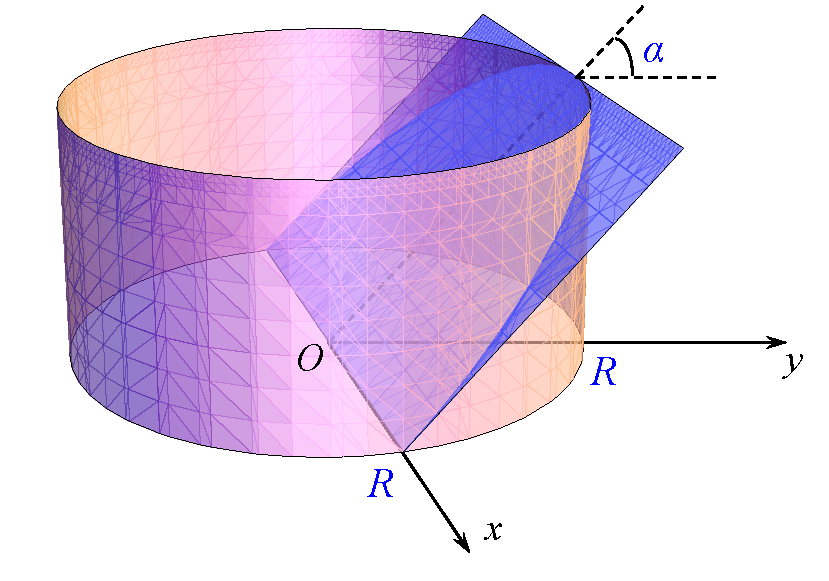
\includegraphics{./images/ch6/bucket.pdf}}
\end{center}

{\bf 例:}半径不等的两个木质球体,分别中间凿去一个以直径为轴的正圆柱体以及柱体下方的球冠,
剩下的环状部分高度均为$h$,问哪一个环状物体的体积更大。

[提示]:
$$V=\dint_{\sqrt{R^2-h^2}}^R2\pi x\sqrt{R^2-x^2}\d x=\df23\pi h^3$$
结果表明:剩余部分的体积与球半径无关!

{\bf 例:}试推导球的体积公式和球面上一块面积为$S$的球心锥的体积公式($rS/3$)

{\bf 例:}开口容器内的水在单位时间内的蒸发量与水的表面积成正比,证明:水的深度以常速率
下降且与容器形状无关。

[提示]:设水的表面积为$S$,则
$$\Delta V\approx S\Delta h\Rightarrow
\df{\Delta V}{\Delta t}\approx S\df{\Delta h}{\Delta t}$$
即
$$\df{\d V}{\d t}=S\df{\d h}{\d t}$$

\subsection{物理应用}

\subsubsection{【平面物体的质心】}
$y=f(x)(a<x<b)$密度均匀,其质心的横坐标为
$$\bar{x}=\df{\dint_a^bxf(x)\d x}{\dint_a^bf(x)\d x}$$

{\bf 例:}求右半圆的质心坐标。

{\bf 例:}$f(x)\in C[a,b]$且单调递增,证明:
$$\dint_a^bxf(x)\d x\geq\df{a+b}2\dint_a^bf(x)\d x$$
[提示]:物理意义:递增函数的形成的曲边梯形质心位于右侧。

证1:由$f(x)$单增,
$$\left(x-\df{a+b}2\right)\left[f(x)-f\left(
\df{a+b}2\right)\right]\geq0$$
两边积分即得。

注:$f\left(\df{a+b}2\right)\dint_a^b\left(x-\df{a+b}2\right)=0$

证2:记$c=\df{a+b}2$
\begin{align}
	\dint_a^b&(x-c)f(x)\d x\notag\\
	&=\left(\dint_a^c+\dint_c^b\right)(x-c)f(x)\d x\notag\\
	&=f(\xi_1)\dint_a^c(x-c)\d x+f(\xi_2)\dint_c^b(x-c)\d x\notag\\
	&=[f(\xi_1)-f(\xi_2)]\df{(b-a)^2}2\geq0
\end{align}

\subsubsection{【变力沿直线做功】}

{\bf 例:}一圆柱形的水桶高$5m$,底半径$3$m,桶内装满水,问要将桶内的水全部抽出,
需要做多少功(设重力加速度$g=10N/kg$)。

{\bf 例:}在由电量为$+q$的电荷产生的电场中,沿某一轴向将一个单位正电荷由距离
$a$移动到距离$b$的位置,问在该过程中,电场力共对该电荷做了多少功?

{\bf 电场力:}
$$F=k\df{q_1q_2}{r^2}$$

\subsubsection{【水压】}

{\bf 例:}某个圆柱形油桶底半径为$R$,所装油密度为$\rho$,
现将其装满油后横放,求其端面承受的压力。

\subsubsection{【万有引力】}

{\bf 例:}设有一长度为$l$,线密度为$\mu$的均匀细直棒,在其中垂线上距离棒$a$
处有一质量为$m$的质点$M$,求该棒对质点$M$的引力。

[提示]:
\begin{align}
	F&=-\dint_{-\frac l2}^{\frac l2}\df{Gam\mu}{(a^2+y^2)^{\frac32}}\d y
	=-\dint_{-\arctan\frac l{2a}}^{\arctan\frac l{2a}}\df{Gam\mu}{(a^2+(a\tan
	t)^2)^{\frac32}}\d (a\tan t)\notag\\
	&=-\df{Gm\mu}a\dint_{-\arctan\frac l{2a}}^{\arctan\frac
	l{2a}}\cos t\d t=-\df{Gm\mu}a\left.\sin t\right|_{-\arctan\frac
	l{2a}}^{\arctan\frac l{2a}}\notag\\
	&=-\df{2Gm\mu}a\sin\left(\arctan\df l{2a}\right)\notag
\end{align}
注意到$\sin x=\df{\tan x}{\sec x}=\df{\tan x}{\sqrt{1+\tan^2 x}}$,故
$$\sin\left(\arctan\df l{2a}\right)=\df{\frac{l}{2a}}
{\sqrt{1+\left(\frac{l}{2a}\right)^2}}=\df{l}{\sqrt{4a^2+l^2}}$$
代回前式即得$F=-\df{2Gm\mu l}{a\sqrt{4a^2+l^2}}$。

\section{反常积分}



\newpage

\section*{课后作业}
\addcontentsline{toc}{section}{课后作业}

{\bf 【必作题】}

\begin{itemize}
  \item 习题6.1:3(2,4),4,5(4,5,6),7
  \item 习题6.2:1(5-8),4,6,8,11,12,13
  \item 习题6.3:4(3,4,5,11,12,15,16),5,6(6,7,8,9),7(5,8,12,16),
  8,11,12(3,4),16
  \item 习题6.4:2,5,6(1),8,10,11,15,16,19
  \item 习题6.5:1(4-6),2,3,6,8
\end{itemize}

\bigskip

\hrule

\bigskip
\bigskip

{\bf 【思考题】}

\begin{itemize}
  \item 习题6.1:9,10
  \item 习题6.2:3,7,9,10
  \item 习题6.3:9,17,18
  \item 习题6.4:1-30其余各题
  \item 习题6.5:4,5
\end{itemize}

% {\bf 例:}$a>0,c\in(0,e^a)$,证明:
% $$\dint_0^a|e^x-c|\dx\geq(e^{\frac a2}-1)^2$$

\newpage

\section*{习题参考解答}
\addcontentsline{toc}{section}{习题参考解答}

{\bf 习题6.5-8.} 长度为$l$的细杆,均匀带电,总电量为$q\,(q<0)$,若在杆的延长线上,
距离杆一端$x_0$处有一单位正电荷。现将单位正电荷从$x_0$处移动到无穷远,试求克服
电场力所作的功。

解:如图,
\begin{center}
	\resizebox{!}{2cm}{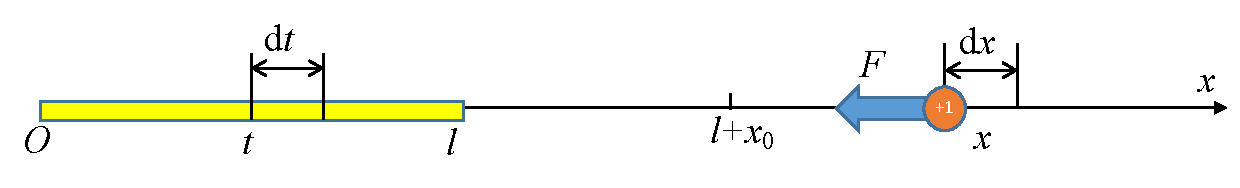
\includegraphics{./images/ch6/eMove.pdf}}
\end{center}

当单位正电荷位于$x(x>l)$处时,细杆上位置$t$处长度为$\d t$的一段对其产生的电场(吸引)力为
$$\d F=\df{kq\d t}{l(x-t)^2},\quad t\in[0,l]$$
故此时单位正电荷所受的总电场力为
$$F=\dint_0^l\df{kq\d t}{l(x-t)^2}=\df{kq}l\left(\df1{x-l}-\df1x\right).$$
克服该力的作用,单位正电荷向远处移动$\d x$,需要做的功为
$$\d W=F\d x=\df{kq}l\left(\df1{x-l}-\df1x\right)\d x,
\quad x\in[l+x_0,+\infty)$$
故所求克服电场力所需做的总功为
$$W=\dint_{l+x_0}^{+\infty}\df{kq}l\left(\df1{x-l}-\df1x\right)\d x
=\df{kq}l\ln\left(1+\df{l}{x_0}\right).$$